%!TEX root = ../dynamics.tex
\section{Large-Scale HIT Type Analysis}\label{sec:type}
In this section we present the results of a large-scale analysis of the evolution of HIT types published on the \amt{} platform.
For such analysis we use the classification of HIT types proposed by \cite{Gadiraju:2014:TMW:2631775.2631819} in which authors perform an extensive study involving 1000 crowd workers to understand their working behavior. 

\subsection{A Classification of HIT Types}
Next, we describe the six top-level classes introduced by \cite{Gadiraju:2014:TMW:2631775.2631819}.

\begin{itemize}

	\item Information Finding (IF): Searching the Web to answer a certain information need. For example, ``Find the cheapest hotel with ocean view in Monterey Bay, CA''.
	
	\item Verification and Validation (VV): Verifying certain information or confirming the validity of a piece of content. Example includes checking twitter accounts for spamming behaviors is a VV task.

	\item Interpretation and Analysis (IA): Interpreting Web content. For example, ``Categorize product pictures in a predefined set of categories'', or ``Classify the sentiment of a tweet''.
	
	\item Content Creation (CC): Generating new content. Examples include summarizing a document  or transcribing an audio recording.

	\item Surveys (SU): Answering a set of questions related to a certain topic (e.g., demographics or customer satisfaction). 
	
	\item Content Access (CA): Accessing some Web content. Examples include watching on-line videos or clicking on provided links.

\end{itemize}

\subsection{Supervised HIT Type Classification}
Using the classification of HIT types described above, we trained a supervised machine learning model to classify HIT type based on their metadata. The features we used to train a Support Vector Machine (SVM) model are title, description, keywords, reward, date, allocated time, batch size.

% labelling setup
To train the supervised model we first created labelled data. We uniformly sampled 5000 HITs over the entire dataset and labelled their type by means of crowdsourcing. In detail, we asked workers on MTurk to assign each HIT to one of the predefined classes by presenting them with the title, description, keywords, reward, date, allocated time, batch size for the HIT. The instructions also contained a definition and examples for each task type. Workers could label tasks as `Others' when unsure or when the HIT did not fit in any of the available options.

% labelled data
After assigning each labelling HIT to three different workers in the crowd, a consensus on the task type was reached in $89\%$ of the cases (i.e., 551 cases with no clear majority). A consensus was reached when at least two out of three workers agreed on a HIT type label. The other cases, that is, when the workers provided different labels or when they where not sure about the label are not included in our labelled dataset.

% classification evaluation
Using the labelled dataset we trained a multi-class SVM classifier for the 6 different task types and evaluated its quality with 10-folds cross validation over the labelled dataset. Overall, the trained classifier obtained Precision of $0.895$, Recall of $0.899$, and F-Measure of $0.895$. Most of the classifier errors (i.e., 66 cases) were done by incorrectly classifying IA instances as CC.

\gd{add top features}

% classification at scale
Using the classifier trained over the entire labelled dataset, we then performed a large scale classification of the type for 2.5M HITs in our collection. This allows us to study the evolution over time of task types on the \amt{} platform which we present next.

\subsection{Task Type Popularity Over Time}
Using the result of the large-scale classification of task types, we can analyze which task types have been published over time.
Figure \ref{fig:cat_trends} shows the evolution of task types published on \amt{}\ .
% 
We can observe that, in general, the most popular type of task is Content Creation.
% 
In terms of observable trends, we note that, while there is a general increase of the volume of tasks of a certain type on the platform,  CA tasks have been decreasing over time. This can be explained for example by the enforcement of \amt{} terms of service which state that workers should not be asked to create accounts on external website or be identified by the requester.
% 
In the last three years, SU and IA tasks have had the biggest increase.

\begin{figure}[htbp]
	\centering
		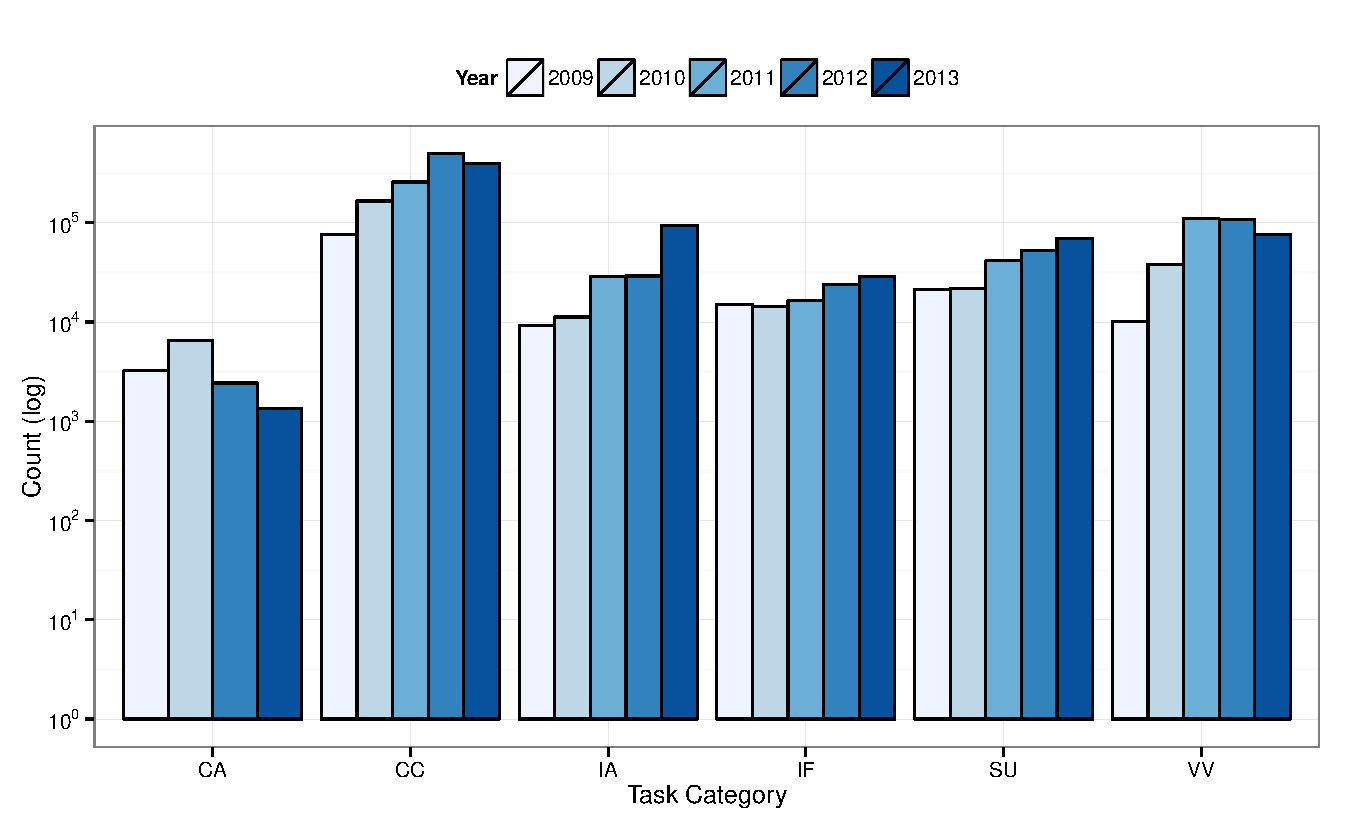
\includegraphics[width=0.5\textwidth]{figures/category_trends}
	\caption{Popularity of HIT types over time. \gd{CA is missing a value? 2011?}}
	\label{fig:cat_trends}
\end{figure}

